\documentclass[../main.tex]{subfiles}

\begin{document}
	\chapter{PID Controller}
	
	\intro{
		PID controller 
	}
	
	
	\begin{section}{Introduction to PID Controllers}
	
	A Proportional-Integral-Derivative (PID) controller is a widely used feedback control mechanism in industrial and engineering systems. It is designed to maintain a desired output by minimizing the error \(e(t)\), which is the difference between a desired setpoint \(r(t)\) and the measured process variable \(y(t)\). The PID controller achieves this by adjusting the control input \(u(t)\) based on three terms: proportional, integral, and derivative.
	The primary motivation for using a PID controller is its ability to regulate dynamic systems efficiently by balancing fast response, minimal steady-state error, and robustness to disturbances. PID controllers are versatile and can be tuned to meet specific performance requirements in diverse applications, such as temperature control, motor speed regulation, and process automation.
	
	\subsection*{Mathematical Details}
	The output of a PID controller, \(u(t)\), is given by:
	
	\[
	u(t) = K_p e(t) + K_i \int_{0}^{t} e(\tau) \, d\tau + K_d \frac{d e(t)}{dt},
	\]
	
	where:
	\begin{itemize}
		\item \(e(t) = r(t) - y(t)\) is the error signal,
		\item \(K_p\) is the proportional gain, controlling the response proportional to the error,
		\item \(K_i\) is the integral gain, reducing steady-state error by integrating the error over time,
		\item \(K_d\) is the derivative gain, predicting future error by calculating the rate of change of the error.
	\end{itemize}
	
	\subsection*{Components of a PID Controller}
	\begin{enumerate}
		\item \textbf{Proportional Term}: \(K_p e(t)\) provides an immediate response proportional to the current error. However, it may not fully eliminate the steady-state error.
		\item \textbf{Integral Term}: \(K_i \int_{0}^{t} e(\tau) \, d\tau\) accumulates past errors, addressing steady-state error by applying corrective action based on the error history.
		\item \textbf{Derivative Term}: \(K_d \frac{d e(t)}{dt}\) predicts future errors by responding to the rate of change of the error, improving stability and damping oscillations.
	\end{enumerate}
	PID controllers are simple to implement, robust, and effective for a wide range of systems. With proper tuning of \(K_p\), \(K_i\), and \(K_d\), they can balance speed, stability, and accuracy in dynamic environments.
	\end{section}




	\begin{section}{PID Contoller in Max Delivery}
		\subsection*{Main Algorithm}
		In \autoref{sec:md_optimal}, we mentioned that, optimally, the amount of budget depleted within a time interval should be proportional to the number of auction opportunities during that time interval, i.e.,

		\[
		\sum_{\tau \leq t \leq \tau + \Delta \tau} x_t c_t \propto \text{\# of auction opportunities in } (\tau, \tau + \Delta\tau).
		\]
		
		Remember that the optimal bid is the bid that just depletes the campaign's budget, assuming there is abundant supply. In practice, we can first construct the target spend per interval and use this target spend as the setpoint to apply the PID controller discussed above. Suppose we have a CPC campaign with a daily budget of \$100. We bucketize one day by choosing the bucket interval $\Delta\tau =$ 15 minutes and obtain the predicted number of eligible requests (auction opportunities) for these intervals from the prediction model, as shown in \autoref{fig:flow_ratio_15min}.
		
		\begin{figure}[H]
			\centering
			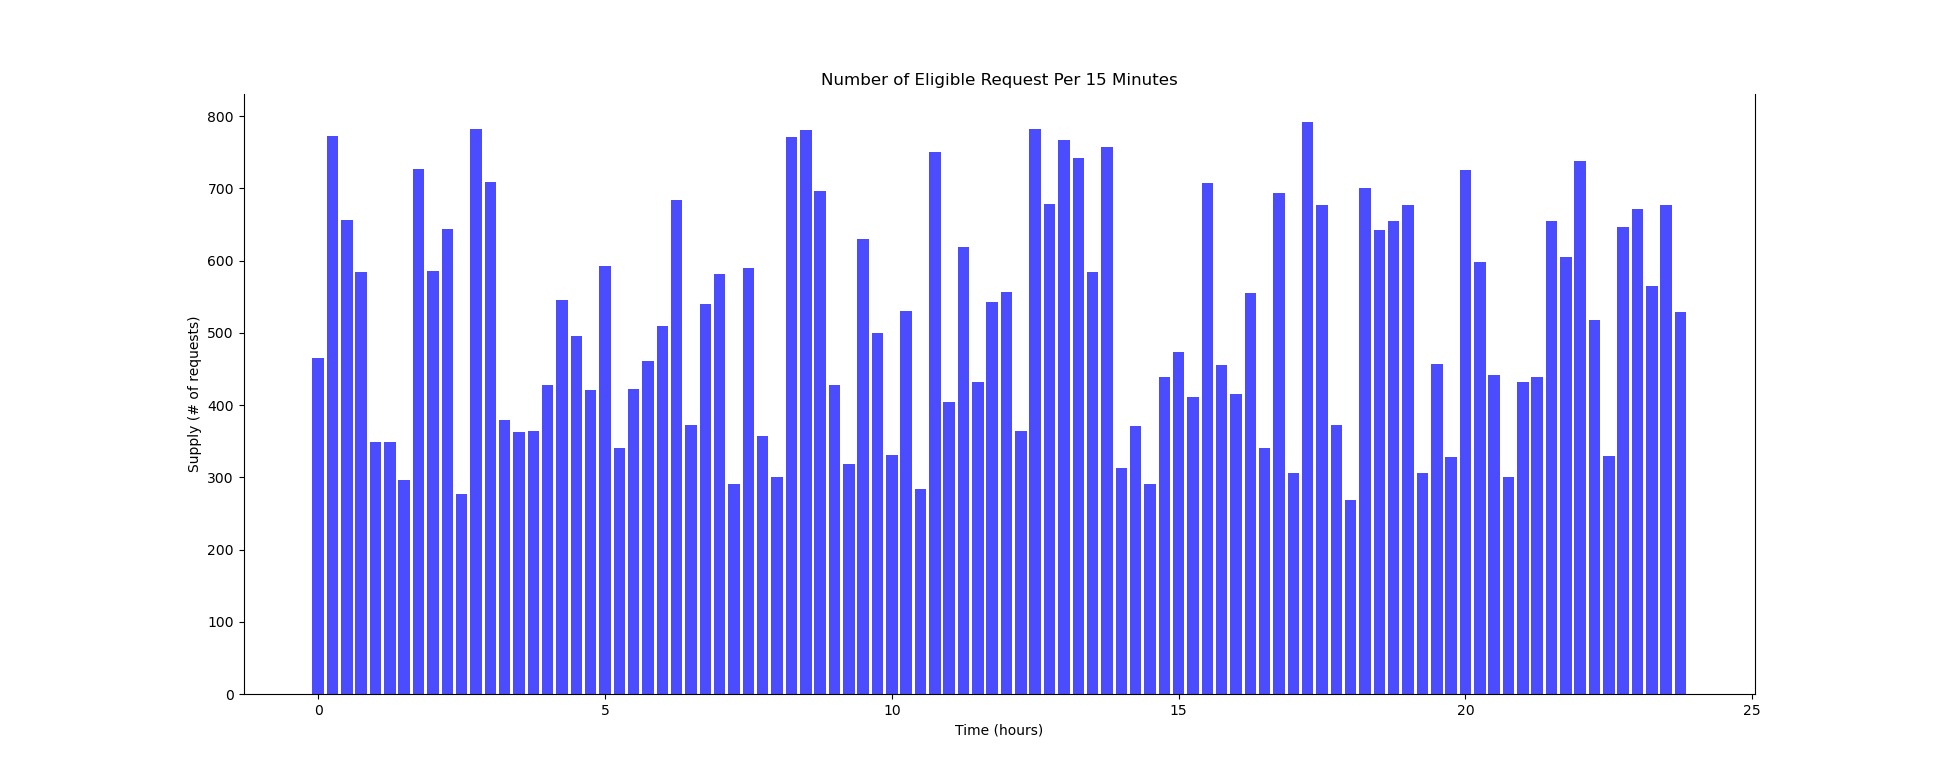
\includegraphics[width=0.99\textwidth]{../Images/flow_ratio_15min.png}
			\caption{Supply Pattern (Number of Eligible Requests Per 15 Minutes)}
			\label{fig:flow_ratio_15min}
		\end{figure}
		
		Based on the supply pattern in \autoref{fig:flow_ratio_15min}, we can construct the target spend per bucket(15-minute interval) for this campaign. For simplicity, within each target spend interval $\Delta\tau$, we assume the budget is consumed linearly over time. Suppose \(TS(t)\) is the target spend in the \(t\)-th interval, \(NR(t)\) is the number of eligible requests in the \(t\)-th interval, \(B = 100\) is the total daily budget, and \(T = 96\) is the number of target spend intervals. The proportional budget allocation rule per interval is given by:
			\[
				TS(t) = \frac{NR(t)}{\sum_{s=1}^{T} NR(s)} \cdot B
			\]
			
		The per-interval target spend is then computed and plotted in \autoref{fig:target_spend_15min}:
		
		\begin{figure}[H]
			\centering
			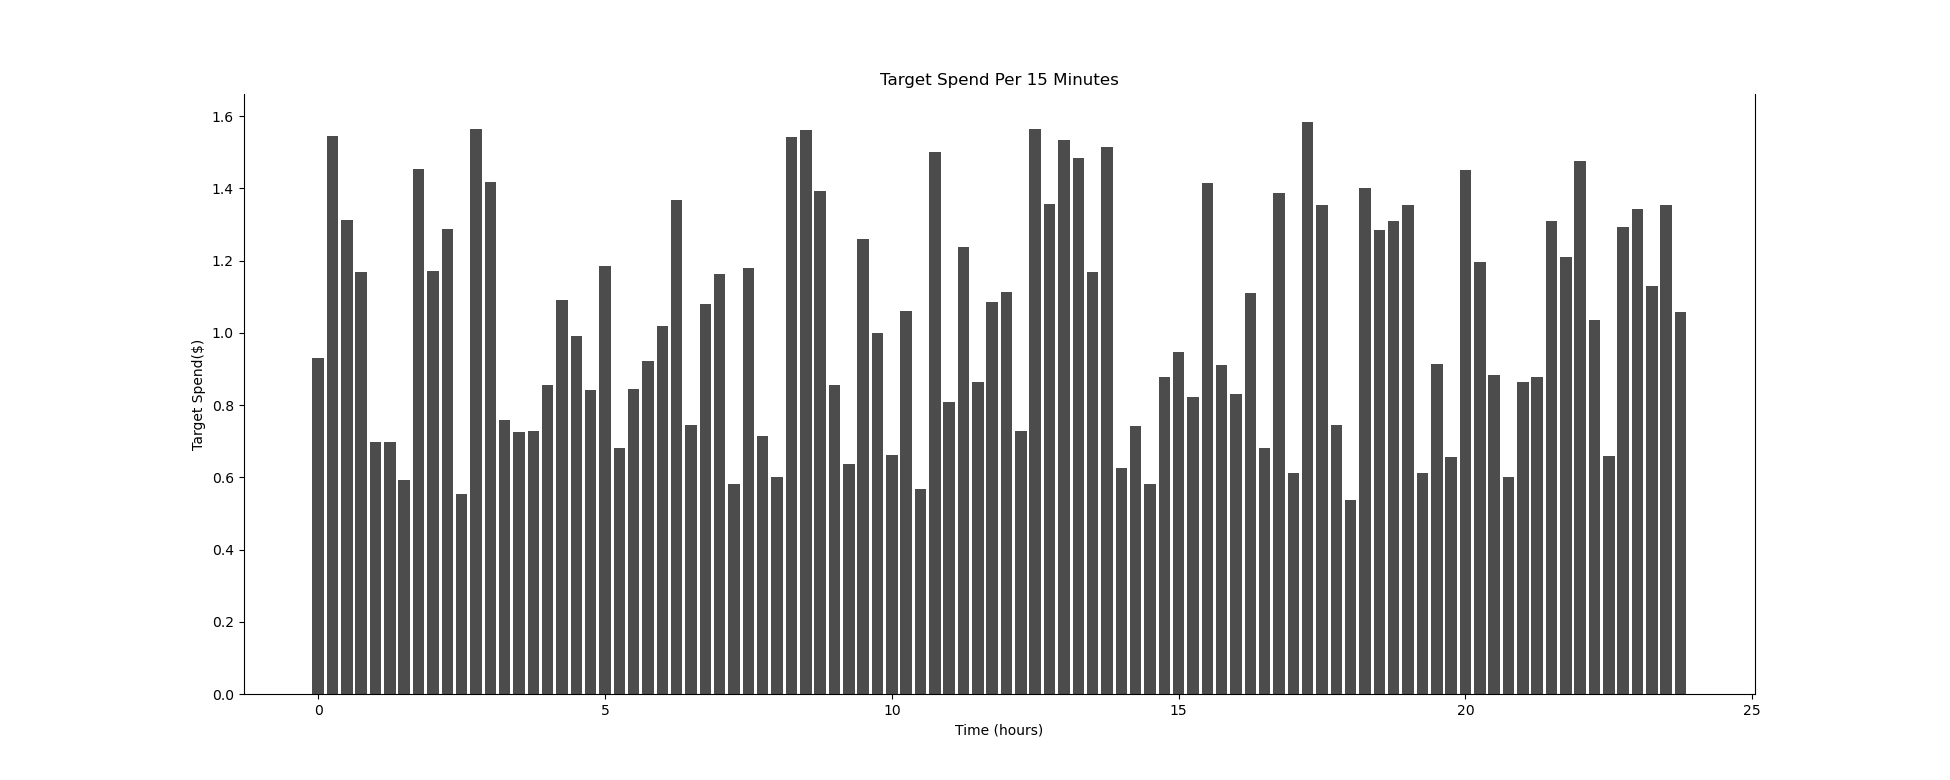
\includegraphics[width=0.99\textwidth]{../Images/target_spend_15min.png}
			\caption{Target Spend Per 15 Minutes}
			\label{fig:target_spend_15min}
		\end{figure}
	
	We summarize the budget allocation algorithm as follows:
	
		\begin{algorithm}[H]
		\caption{Compute Target Budget per Bucket}
		\begin{algorithmic}[1]
			\Require $B$: Total daily budget
			\Require $NR(t)$: Number of eligible requests in interval $t$
			\Require $T$: Total number of buckets in a day
			\State Initialize $TS(t) \gets 0$ for all $t = 1, \dots, T$
			\State Compute the total eligible requests:
			\[
			\text{TotalRequests} \gets \sum_{t=1}^{T} NR(t)
			\]
			\For{$t = 1$ to $T$}
			\State Compute the proportional share of the budget for bucket interval $t$:
			\[
			TS(t) \gets \frac{NR(t)}{\text{TotalRequests}} \cdot B
			\]
			\EndFor
			\State \Return $TS(t)$ for all $t = 1, \dots, T$
		\end{algorithmic}
	\end{algorithm}
	
		Suppose the bid price gets updated every \(\Delta t\) time (\(\Delta t\) is a tunable bid update interval, which we may set to, e.g., 1 minute) at \(t_0, t_1, t_2, \cdots, t_N\), where \(N = \text{MinutesInOneDay} / \Delta t\). We define the error factor and control signal as:
		
		\[
		\begin{aligned}
			e(t_k) &= r_{t_k} - s(t_k), \\
			u(t_{k}) &\gets K_p e(t_k) + K_i \sum_{j=1}^{k} e(t_j) \Delta t + K_d \frac{\Delta e(t_k)}{\Delta t},
		\end{aligned}
		\]
		
		where:
		\begin{itemize}
			\item \(r_{t_k}\): Observed spend during the \(k\)-th pacing update interval,
			\item \(s(t_k)\): Target spend derived by proportionally allocating within the target budget interval \(\Delta\tau\) that contains it, e.g., if \([t_{k-1}, t_k]\) lies within the \(t\)-th target budget interval, then 
			\[
			s(t_k) = \frac{\Delta t}{\Delta\tau} \cdot TS(t),
			\]
			where \(TS(t)\) is the target spend for the \(t\)-th interval.
			
		\end{itemize}
		
		The bid can be updated by leveraging an actuator that takes the current control signal \(u(t_k)\) to adjust the current bid price \(b(t_k)\) as:
		
		\[
		b(t_{k+1}) \gets b(t_k) \exp\{u(t_{k})\}.
		\]
		
		The PID algorithm for max delivery problem is summarized in \autoref{alg:pid_md}. For more in-depth knowledge on applying PID controllers to the max delivery pacing problem, one may refer to  \cite{wang2017display} and \cite{zhang2016feedback}.
		
		\begin{algorithm}
			\caption{PID Controller for Bid Price Modulation in Max Delivery}
			\label{alg:pid_md}
			\begin{algorithmic}[1]
				\Require $\Delta t$: Time interval for bid updates(e.g. 1 minute)
				\Require $T$: Total campaign duration
				\Require $B$: Total campaign budget
				\Require $\Delta \tau$: Time interval of target budget per bucket
				\Require $\{ TS(t) \}$: Target spend for each target budget interval $t$
				\Require $K_p, K_i, K_d$: PID controller gains
				\State Initialize $b(t_0) \gets \text{initial\_bid}$
				\State Initialize $u(t_0) \gets 0$
				\State Initialize $\text{cumulative\_error} \gets 0$
				\State Initialize $\text{previous\_error} \gets 0$
				
				\For{$k = 1$ to $N$} \Comment{$N = \text{MinutesInOneDay} / \Delta t$}
				\State Find the $t$-th target budget interval that contains $t_k$ update interval, compute:
				\[
				s(t_k) \gets \frac{\Delta t}{\Delta\tau} \cdot TS(t)
				\]
				\State Measure observed spend during the interval:
				\[
				r(t_k) \gets \text{observed\_spend}(t_k)
				\]
				\State Compute the error factor:
				\[
				e(t_k) \gets r(t_k) - s(t_k)
				\]
				\State Update the control signal using the PID formula:
				\[
				u(t_k) \gets K_p \cdot e(t_k) + K_i \cdot \text{cumulative\_error} + K_d \cdot \frac{e(t_k) - \text{previous\_error}}{\Delta t}
				\]
				\State Update the cumulative error:
				\[
				\text{cumulative\_error} \gets \text{cumulative\_error} + e(t_k) \cdot \Delta t
				\]
				\State Update the bid price:
				\[
				b(t_k) \gets b(t_{k-1}) \cdot \exp(u(t_k))
				\]
				\State Update the previous error:
				\[
				\text{previous\_error} \gets e(t_k)
				\]
				\State Actuate the new bid price:
				\[
				\text{submit\_bid}(b(t_k))
				\]
				\EndFor
			\end{algorithmic}
		\end{algorithm}
		
		\subsection*{Bidding Dynamics}
		We show here the detailed bidding dynamics for this campaign. \autoref{fig:flow_ratio_map} is a simplified plot demonstrating how the PID controller operates in a real-world dynamic environment. 
		\begin{figure}[H]
			\centering
			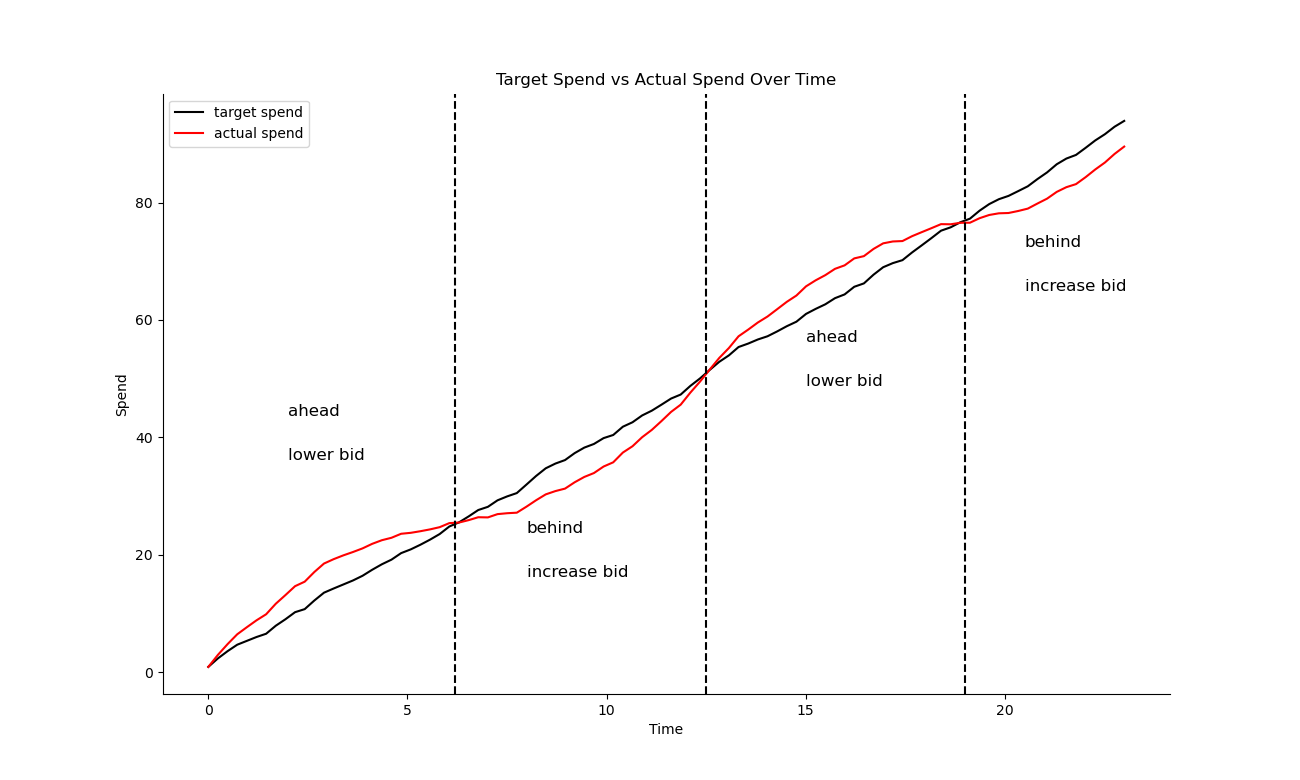
\includegraphics[width=0.99\textwidth]{../Images/flow_ratio_map.png}
			\caption{Target Spend vs Actual Spend Over Time}
			\label{fig:flow_ratio_map}
		\end{figure}
	The dynamics of a PID controller adjusts bids based on the relationship between the \textbf{target spend} (black line) and the \textbf{actual spend} (red line) over time. Target spend represents the ideal cumulative budget spending at any point in time to evenly distribute the budget. Actual spend reflects the real cumulative spend achieved by the campaign over time.  The graph highlights two key conditions: being \textbf{ahead of the schedule} or \textbf{behind the schedule}, and how these conditions affect bid modulation.
	
	If the delivery is behind the schedule, i.e. when the actual spend (red line) is below the target spend (black line), the campaign is under-delivering. The PID controller \textbf{increases the bid} to catch up with the target spend. Higher bids make the campaign more competitive in auctions, increasing the likelihood of winning more impressions and spending more. In the plot, the actual spend curve slopes upward more steeply after the "increase bid" label in the "behind" regions; If the delivery is ahead of the schedule, i.e. when the actual spend (red line) exceeds the target spend (black line), the campaign is over-delivering. The PID controller \textbf{lowers the bid} to slow down the spending rate and realign with the target spend. Lower bids reduce the competitiveness of the campaign in auctions, resulting in fewer impressions and slower spend. In the plot, the actual spend curve becomes less steep after the "lower bid" label in the "ahead" regions.
	
	This feedback mechanism ensures a balanced distribution of the budget over time, optimizing performance while adhering to pacing constraints.
	
	\subsection*{Practical Considerations}
	We list here some practical considerations for implementing the PID controller in real-world production sytem:
	\begin{itemize}
		\item \textbf{Normalization of error signal}: The error factor \(e(t_k)\) in \autoref{alg:pid_md} is defined as \(r(t_k) - s(t_k)\), the gap between actual spend and target spend. However, the issue is that the scale of the budget varies significantly across different campaigns, requiring different controller gains to accommodate these budget fluctuations. In practice, it is challenging to maintain different controller gains for each campaign, and it is more common for all ad campaigns to share the same controller gains. In this situation, a better approach is to compute the error factor in a normalized way, i.e.,
		\[
		e(t_k) = 1 - \frac{r(t_k)}{s(t_k)},
		\]
		which normalizes the error factors for campaigns with different budget scales to a common scale.
		\item \textbf{Different Actuator}: The update rule in \autoref{alg:pid_md} is \(b(t_k) \gets b(t_{k-1}) \cdot \exp(u(t_k))\), where the \(\exp\) function is chosen as the actuator. In practice, other functions can also be used as the actuator function, such as linear functions or sigmoid functions.
		
		\item \textbf{Choice of \(\Delta \tau\) and \(\Delta t\)}: Some trade-offs should be considered when choosing the target spend bucket \(\Delta \tau\) and the bid update interval \(\Delta t\). 
		
		\begin{itemize}
			\item \textbf{Target Spend Bucket \(\Delta \tau\)}: 
			\begin{itemize}
				\item A small \(\Delta \tau\) provides finer-grained predictions of the supply pattern, reducing the accuracy requirements for interpolation within the bucket. However, the prediction itself may become noisier.
				\item A large \(\Delta \tau\), on the other hand, gives a more accurate estimate of the overall supply. However, the assumption of a linear distribution of supply within \(\Delta \tau\) is less likely to hold, which can negatively impact interpolation accuracy.
			\end{itemize}
			\item \textbf{Bid Update Interval \(\Delta t\)}:
			\begin{itemize}
				\item A small \(\Delta t\) results in more responsive updates to the market, but the computed error factor may contain more noise.
				\item A large \(\Delta t\) helps mitigate statistical noise in the error factor, but delayed bid updates may fail to respond to market changes in a timely manner.
			\end{itemize}
		\end{itemize}
		
		These two parameters can be tuned online. In practice, we find that setting \(\Delta \tau\) to a duration ranging from a few minutes to an hour, and setting \(\Delta t\) to a comparable range, typically works well.
		
	\end{itemize}
	
	\end{section}
	
	
	\begin{section}{PID Contoller in Cost Cap}
		cost-min paper: \cite{kitts2017ad}
		
	\end{section}
	
	
\end{document}
